\section{Semantic Modeling of Computational Resources}
\label{sec:semantic}

Scientific workflows are also used for preserving and sharing scientific experiments 
in science. Research efforts focused on describing the workflow structure and the 
experimental data, both input data and results. In this work, we argue that the information 
about the computational resources should be also provided for achieving full reproducibility. 
These descriptions allow the target audience, usually another scientist in the same domain, 
to understand the underlying components involved in a workflow execution.

We propose the definition of semantic models for describing the main domains of a 
computational infrastructure, and for defining the taxonomy of concepts and the relationships 
between them. These models describe the software components, hardware specifications, 
and the available computational resources (in the form of VMs). They also capture infrastructure 
dependencies of the workflows. As a result, this process facilitates experiment's reusability since 
a new experiment, which may reuse parts of the workflow previously modeled, or a reproduction 
of a workflow, would benefit from the infrastructure dependencies already described.

We have identified four main domains of interest for documenting computational scientific 
infrastructures~\cite{wicus}. We have developed a set of models, one for each domain, 
and an ontology network that defines the inter-domain relations between these models 
(Figure~\ref{fig:wicusrels}):

\begin{figure}[!b]
	\centering
	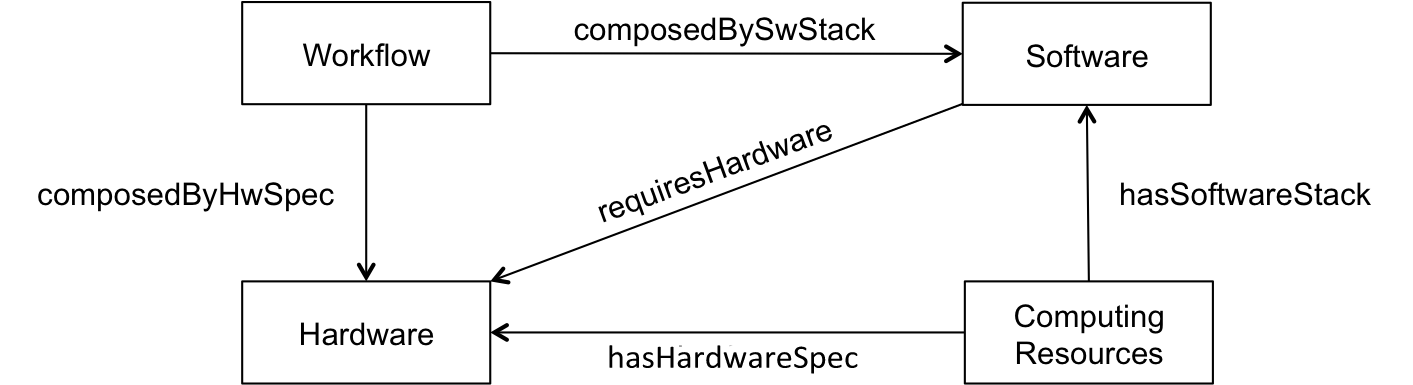
\includegraphics[width=.9\linewidth]{figures/wicusrels}
	\caption{Overview of the ontology network ($\rightarrow$ denotes inter-domain relation).}
	\label{fig:wicusrels}
\end{figure}

\begin{itemize}
	\setlength{\itemsep}{1pt}
	\setlength{\parskip}{0pt}
	\setlength{\parsep}{0pt}

	\item{\emph{Hardware domain}}: identifies the most common hardware information, 
		including CPU, Storage and RAM memory, and their capacities.
	
	\item{\emph{Software domain}}: defines the software components involved on the execution. 
    		It includes the pieces of executable software (e.g., scripts, binaries, and libraries) used in 
		the experiment. In addition, dependencies between those components and configuration 
		information are also defined, as well as the required steps for deploying them.
	
	\item{\emph{Workflow domain}}: describes and relates workflow fragments (a.k.a transformations) 
    		to their dependencies. Therefore, scientists can understand what are the relevant infrastructure 
		components for each part of the workflow.
	
	\item{\emph{Computing Resources domain}}: expresses the information about the available 
    		computing resources. In this domain, only virtualized resources are currently considered 
		(i.e., virtual machine). It includes the description of the VM image, its provider, and specifications.
\end{itemize}